\documentclass[a4paper]{article}
\usepackage[german]{babel}
\usepackage[utf8]{inputenc}
\usepackage{amsmath}
\usepackage{amssymb}
\usepackage{graphicx}
\usepackage{float} 
\usepackage{verbatim} 
\graphicspath{ {images/} }
\title{Operating System Lab 1}
\author{
	Pfeffer, Moritz 
	\texttt{3261671}
	\and
	Liao, Fangwen
	\texttt{3439869}
	\and
	Wang, Yijin
	\texttt{3476217}
} 

\begin{document}
	\maketitle
	\section*{1}
	\subsection*{(a)}
	\begin{itemize}
		\item{your answer}
		\item{your answer}
			\begin{figure}[h]
				\centering
				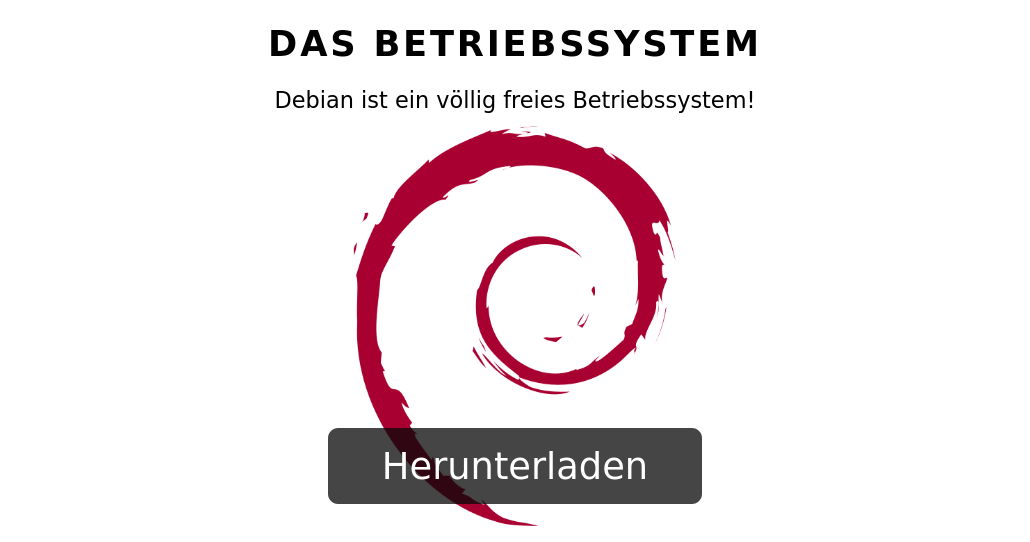
\includegraphics[width=5cm, height=2cm]{screenshot0.png}
				\caption{The first picture}
			\end{figure}
		\item{your answer}
		
	\end{itemize}

	\subsection*{(b)}
	\begin{itemize}
		\item{your answer}
	\end{itemize}
	
	\section*{2}
	\subsection*{(a)}
	\begin{itemize}
		\item{your answer}
		\item{your answer}
			\begin{table}[h]
				\centering
				\begin{tabular}[h]{|c|c|c|}
					\hline
					cell1 & cell2 & cell3 \\ 
					\hline
					cell4 & cell5 & cell6 \\  
					\hline
					cell7 & cell8 & cell9 \\   
					\hline
				\end{tabular}
				\caption{A table}
			\end{table}
		
		\item{your answer}
		\item{your answer}
		
	\end{itemize}
	\begin{center}
		
	\end{center}
	\subsection*{(b)}
	
	\section*{3}
	\subsection*{(a)}
	\begin{itemize}
		\item{your answer\cite{handbook}}
	\end{itemize}
	
	\subsection*{(b)}
	
	\section*{4}
	\subsection*{(a)}
	\subsection*{(b)}
	
	
	
	\begin{thebibliography}	{}
		\bibitem{handbook} Robert Love, Linux Kernel Handbuch, 2005.		
	\end{thebibliography}
\end{document}